\section{Introducción a tipos sesión}

\begin{frame}{Índice}
	\tableofcontents[currentsection] \note{Primero introducción a qué son y
	qué problema buscan resolver los tipos sesión. Después charlar sobre la
	variante probabilística. Luego el objetivo de este trabajo y un paseo
	por el mismo.}
\end{frame}

\begin{frame}{\insertsection}

	El desarrollo de software distribuido se enfoca principalmente en la
	integración, cooperación y comunicación de componentes en un sistema.

	\bigskip

	Dificultades:
	\begin{itemize}
		\item{Desafío tecnológico}
		\item{\alert<2>{Razonamiento sobre el sistema}}
		\pause
	\end{itemize}

	\note{Desafío tecnológico: trabajo correspondiente a la
	integración concreta de los componentes. Implementación.
	\\
	Razonamiento: comprender el estado de un sistema distribuido.}
\end{frame}

\begin{frame}{\insertsection}
	\begin{figure}
		\centering
		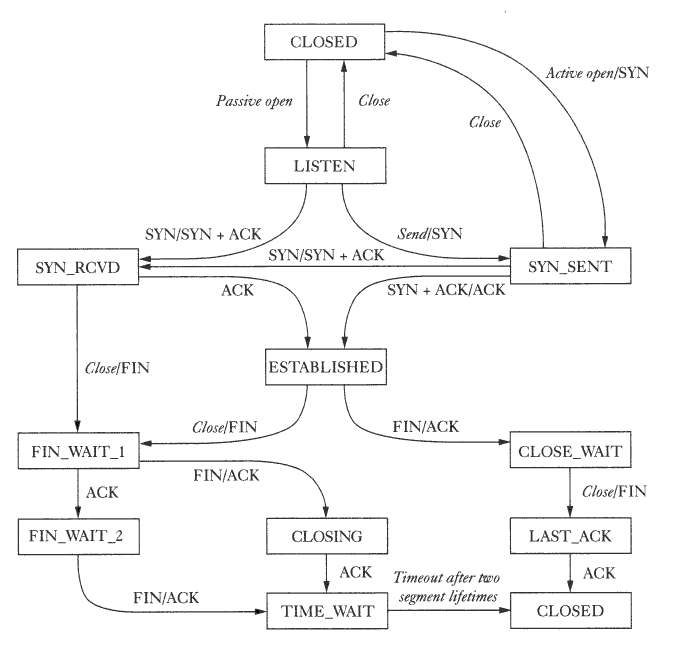
\includegraphics[width=0.6\textwidth]{images/tcp-state-diagram.png}
		\caption{Diagrama de estados para protocolo \textsc{TCP}}
	\end{figure}
	\note{Mostrar brevemente como ejemplo de la complejidad que puede tener un sistema distribuido en términos de estados posibles y propiedades a lo largo de los mismos}
\end{frame}

\begin{frame}{\insertsection}

	Esto dio lugar a:

	\begin{itemize}
		\item Desarrollo de técnicas de descripción de interfaces
		\item Soporte a nivel de lenguajes de programación para el desarrollo de aplicaciones correctas por construcción
	\end{itemize}

	\pause

	Los tipos comportamentales, tales como los \textbf{tipos de sesión} constituyen
	un ejemplo paradigmático de esta línea de trabajo.
\end{frame}

\begin{frame}{\insertsection}
	Los tipos de sesión proponen estructurar la
	comunicación entre componentes alrededor del concepto de \textbf{sesión}.

	\begin{itemize}
		\item Una sesión es un canal privado que permite
			conectar a dos (a veces más) procesos.

		\item Cada proceso posee un \textbf{endpoint} de la sesión y lo
			debe usar siguiendo un protocolo bien especificado
			(tipo sesión) que restringe la secuencia de mensajes
			que se pueden enviar y recibir a través del mismo.
	\end{itemize}

	\begin{figure}
		\centering
		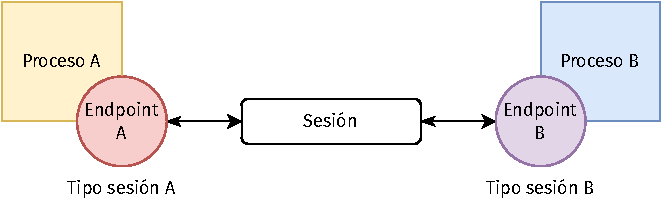
\includegraphics[width=0.8\textwidth]{images/tipo-sesion.pdf}
		\caption{Estructura de comunicación mediante tipos sesión}
	\end{figure}
\end{frame}

\subsection{Ejemplo: Describiendo suma con tipos sesión}

\begin{frame}{\insertsubsection}
	Consideremos un protocolo básico para la suma de dos números:
	\begin{enumerate}
		\item Cliente envía primer sumando
		\item Cliente envía segundo sumando
		\item Servidor retorna suma
	\end{enumerate}
\end{frame}

\begin{frame}{\insertsubsection}
	\begin{figure}
		\centering
		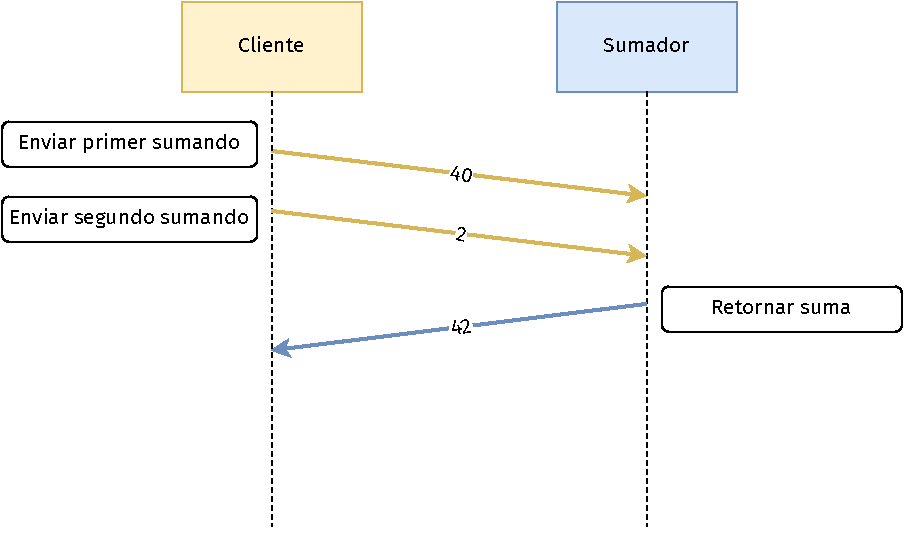
\includegraphics[width=0.9\textwidth]{images/sum-diagram.pdf}
		\caption{Ejemplo de comunicación para servicio sumador}
	\end{figure}
\end{frame}

\begin{frame}{\insertsubsection}
	\begin{figure}
		\centering
		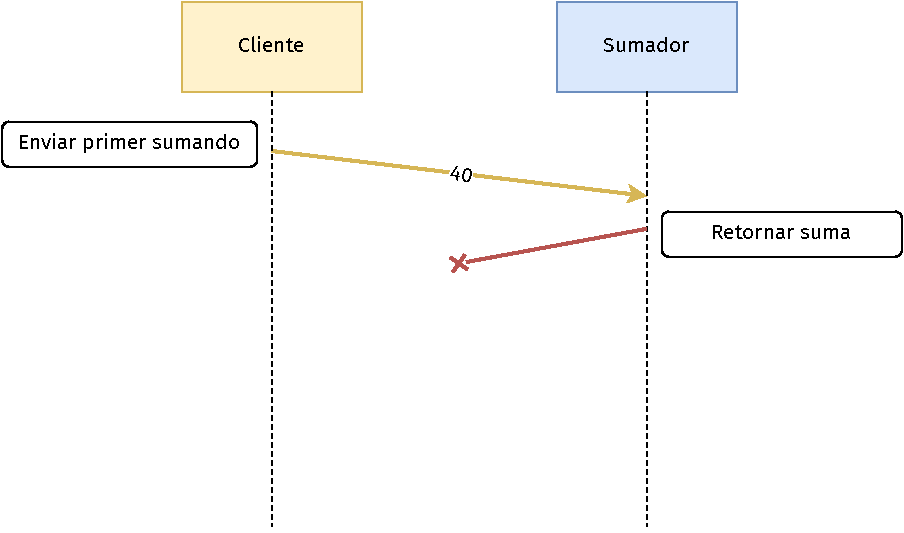
\includegraphics[width=0.9\textwidth]{images/sum-diagram-illegal.pdf}
		\caption{Violación de linearidad}
	\end{figure}
\end{frame}

\begin{frame}{\insertsubsection}
	\begin{figure}
		\centering
		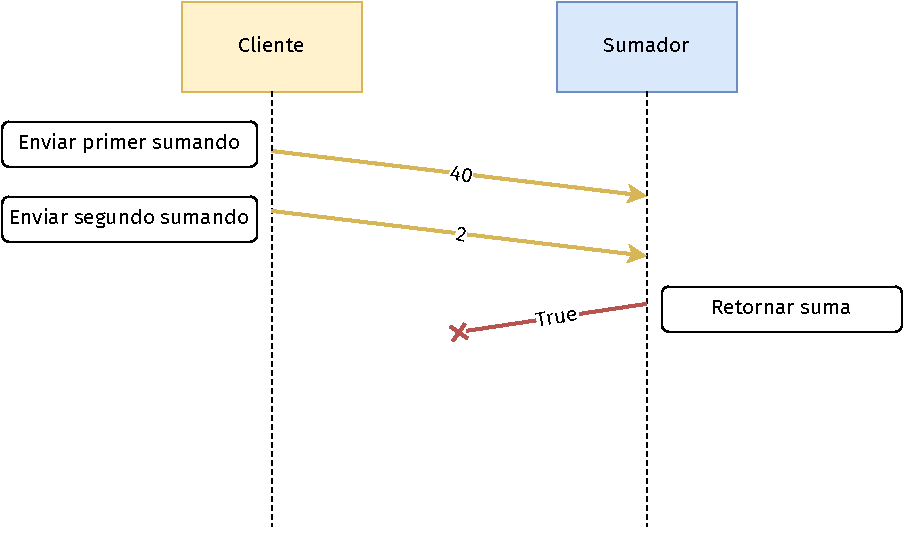
\includegraphics[width=0.9\textwidth]{images/sum-diagram-type-violation.pdf}
		\caption{Tipo de valor de retorno inválido}
	\end{figure}
\end{frame}

\begin{frame}{\insertsubsection}
	Para este ejemplo, la comunicación podría estructurarse mediante los siguientes tipos sesión:
	\begin{itemize}
		\item \textbf{Cliente:} $\SessionType = \Out\tint{ \Out\tint{ \In\tint\End } }$
		\item \textbf{Sumador:} $\dual\SessionType = \In\tint{ \In\tint{ \Out\tint\End } }$
	\end{itemize}

	\begin{figure}
		\centering
		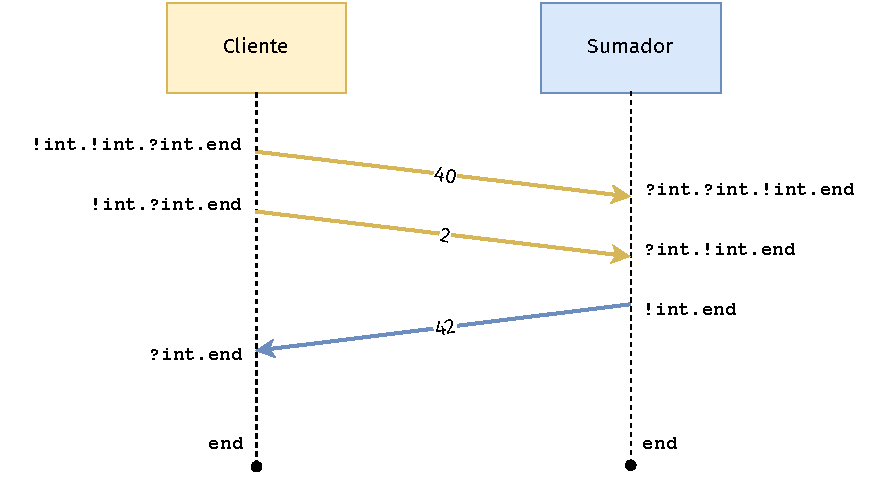
\includegraphics[width=0.9\textwidth]{images/sum-diagram-st.pdf}
	\end{figure}
\end{frame}

\subsection{Implementación de tipos sesión: FuSe}

\begin{frame}{\insertsubsection}
	\FuSe es una biblioteca que habilita el uso de tipos sesión binarios en
	\OCaml.
	\begin{itemize}
		\item Codificación basada en igualdad de tipos y tipos parametrizados.
		\item Detección de violaciones de linearidad en tiempo de ejecución.
		\item Garantiza comunicación segura, fidelidad y progreso (siempre y cuando no haya deadlocks y se respete la linearidad).
		\item Inferencia de tipos y subtipado provisto por el sistema de tipos de \OCaml.
	\end{itemize}
	\begin{figure}
		\centering
		
\includegraphics[width=0.3\textwidth]{images/ocaml-logo.png}
	\end{figure}
\end{frame}

\begin{frame}{\insertsubsection}
	\SumClient
	Evolución del tipo sesión:
	\begin{itemize}
		\item \OI{ep0:} $\Out\tint{ \Out\tint{ \In\tint\End } }$
		\item \OI{ep1:} $\Out\tint{ \In\tint\End }$
		\item \OI{ep2:} $\In\tint\End$
		\item \OI{ep3:} $\End$
	\end{itemize}
\end{frame}
\begin{frame}{\insertsubsection}
	\SumServer
	Creamos un \emph{thread} con el sumador y realizamos una suma con el cliente:
	\SumExample
\end{frame}
